\chapter{Requirements Analysis}
\label{sec:requirements}
In this chapter our requirement elicitation is provided. Here we discuss the elements the client wants to see back in the end-product. For this purpose the client, who also took the role of supervisor upon himself together with the Tribler team, was interviewed. The requirements that were gathered from this interview were supplemented with additional requirements from our side to complete the product. The requirements were separated into functional and non-functional requirements. Then, use cases for our application were designed, which correspond with the clients wishes. In this phase, a business class diagram was also made which is easier to understand for the client than the complete class diagram of the whole application. 
After researching the framework present on the Samsung SmartTV and the possibilities of libswift, a design for the software architecture could be made. 
Lastly, implementation models such as sequence diagrams and class diagrams were made, which serve as blueprints for the application. Also a MosCoW model was made where the priority off the features to be implemented are stated.

\section{Requirements}
The requirements can be split in two kinds, functional and non-functional requirements. These requirements  correspond to the use cases as mentioned in section \hyperref[sec:use_cases]{\ref*{sec:use_cases}}. The non-functional requirements can then again be split in quality and platform requirements. In this section, the constraints the application has to deal with are also discussed.

\subsection{Functional requirements}
Functional requirements specify the core functionality of the application. These requirements are covered by the use cases in the next section. The functional requirements are as follows:

\begin{itemize}
\item[1.] By using the libswift protocol, given two peers \textit{A} and \textit{B}:
	\begin{itemize}
	\item[1.1.] \textit{A} is able to download from \textit{B} (UC 12);
	\item[1.2.] \textit{A} is able to upload to \textit{B} (Should happen automatically after download is finished);
	\item[1.3.] \textit{A} is able to stream to/from \textit{B} (UC 11);
	\end{itemize}
\item[2.] The users should be able to search for files other peers own by using dispersy (UC 9, 10);
\item[3.] The users should be able to search/browse files they own themselves (UC 2, 8, 10);
\item[4.] The users should be able to playback media content. 
		  Media in this context means any kind of video or audio file supported by the TV (UC 6);
\item[5.] Users should be able to:
	\begin{itemize}
	\item[5.1.] Move files on the file system (UC 5);
	\item[5.2.] Edit files on the file system, i.e. rename files (UC 3);	
	\item[5.3.] Remove files on the file system (UC 4);
	
	\end{itemize}
\item[6.] Users should be able to sort files by name, size, date and type (UC 13, 14, 15, 16, 17); 
\item[7.] Users should be able to separate private files from public files (UC 7);
\item[8.] Users should be able to limit the upload/download speed (UC 1). 
\end{itemize}

\subsection{Non-functional requirements}
Non-functional requirements are those requirements that have to do with the operation of the system. 
Unlike functional requirements, they do not describe what the services the system should provide, 
but more how the system should work. We identified two kinds of non-functional requirements for our application, 
quality and platform requirements.

\subsubsection{Quality requirements}
\begin{itemize}
\item[9.] The response time of the system should be as low as possible since TVs are real-time systems.
We aim to limit the response time to 300 ms;
\item[10.] The RAM memory used by the application should not exceed 256 MB.
This includes the size of the application itself and the memory needed for calculations;
\item[11.] The application may use 100\% CPU power since no other applications should run along the application 
to be built;
\item[12.] Downloads should be continued without loss of data after a failure;
\item[13.] Unfinished downloads should be resumed at start up;
\item[14.] The application should be able to cope with external devices,
memory sticks and other external storage devices in particular;
\item[15.] The user should be able to make use of (part of) the application at any time,
even when no Internet connection is available.
\end{itemize}

\subsubsection{Platform requirements}
\begin{itemize}
\item[1.] The C++ back-end which makes use of the libswift library should be implemented so 
that it is reusable for other systems that work with other front-ends (such as Android);
\item[2.] The application is made to run on a rooted Samsung SmartTV.
To see whether a Samsung TV is rootable or not, please check \url{http://www.samygo.tv/};
\end{itemize}

\subsection{Constraints}
The constraints specify what our own limitations are we have to take into account when implementing the application. 
These can be limitations put by the software we use,
or put by ourselves to reduce the application\textquotesingle s complexity.

\begin{itemize}
\item[1.] Due to the limited memory available on the TV, it is not
possible to download and store great amounts of data on the TV.
Therefore, usage of external storage devices is mandatory to make use
of the application;

\item[2.] The application must be integrated with the Samsung
framework, meaning that it should be recognised by the TV as
JavaScript app developed with the Samsung SDK.
\end{itemize}

\section{Use Cases}
\label{sec:use_cases}
The use case models describe interactions between one or more actors and the system.
The models are used to depict what the users can do with the system and how they  should operate it.
In our case, we only have one actor, which is the user who watches TV. This is because our application should always
maintain the same behaviour for everyone who uses it; everyone using the application has the same rights, privileges
and use cases of the system. The use cases are shown in figure \ref{fig:use_case_diagram},
in which the relations between them are also shown. The user should be able to carry out all the use cases,
these relations are left out for clarity. The use cases in figure \ref{fig:use_case_diagram}
are explained in further detail in their descriptions and with the use of UML sequence diagrams in sections
\hyperref[sec:use_case_descriptions]{\ref*{sec:use_case_descriptions}} and
\hyperref[sec:req_dynamic_models]{appendix} respectively.

\begin{center}
\begin{figure}[h]
	\centering
	\mbox{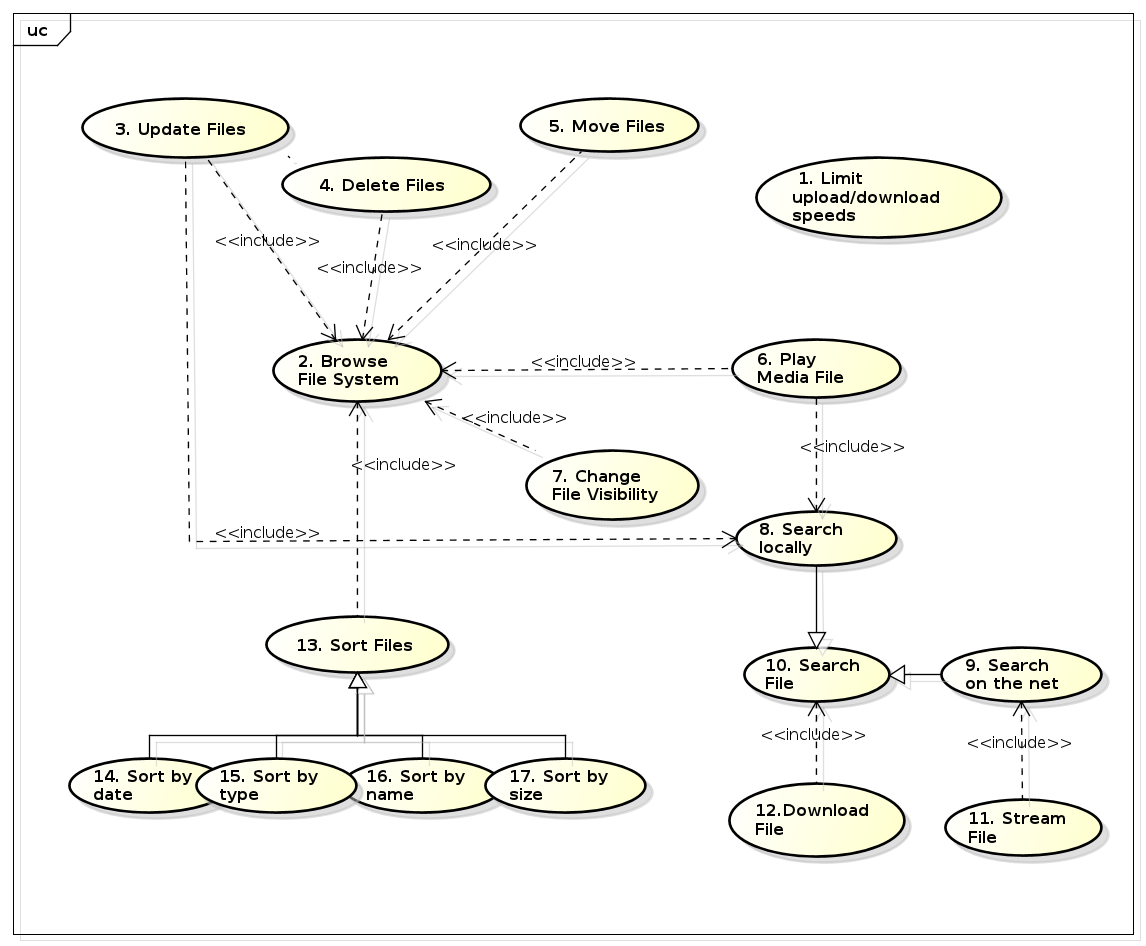
\includegraphics[width=1.2\textwidth]{Images/use_case.png}}
	\label{fig:use_case_diagram}
	\caption{Use case diagram of the application to be built.
	Note that the associations from the user to the use cases are left out in order to keep the diagram clear.}
\end{figure}
\end{center}

\clearpage
\subsection{Use Case Descriptions}
\label{sec:use_case_descriptions}

\begin{table}[h!]
\centering
\begin{tabular}{|l|l|}
\hline
Name & Limit upload/download speeds\\ \hline
Goal & Save bandwidth and memory.\\ \hline
Preconditions & -- \\ \hline
Summary & The user adjusts the upload or download speed.\\ \hline
Steps &  1. User clicks the settings button; \\
      &  2. \textit{System} shows the settings page; \\
      &  3. User sets the download and upload speeds; \\
      &  4. User clicks OK button; \\
      &  5. \textit{System} saves the settings and applies the new speeds;
        \\ \hline
Postconditions & Downloads and uploads will never exceed the new speeds.
\\ \hline
\end{tabular}
\caption{Use Case 1: Limit upload/download speeds. See \hyperref[fig:req_seq1]{appendix} for the sequence diagram.}
\label{tab:UC1}
\end{table}

\begin{table}[h!]
\centering
\begin{tabular}{|l|l|}
\hline
Name & Browse File System\\ \hline
Goal & Getting an overview of the files in the file system.\\ \hline
Preconditions & One or more external storage devices are connected. \\ \hline
Summary & The user browses through the directories on the file system.\\ \hline
Related Cases & Play Media File, Move File, Update File, Delete File, \\ 
              &  Sort Files, Change File Visibility. \\ \hline
Steps &  1. User selects the device to browse; \\
      &  2. \textit{System} shows list of files and directories of the selected device. 
        \\ \hline
Postconditions & -
\\ \hline
\end{tabular}
\caption{Use Case 2: Browse File System. See \hyperref[fig:req_seq2]{appendix} for the sequence diagram.}
\label{tab:UC2}
\end{table}

\begin{table}[h!]
\centering
\begin{tabular}{|l|l|}
\hline
Name & Update Files\\ \hline
Goal & Change the properties of a file.\\ \hline
Preconditions & A changeable file is available locally. \\ \hline
Summary & The user changes the properties of a local file.\\ \hline
Related Cases & Includes \textbf{Browse File System} and \textbf{Search locally}. \\ \hline
Steps &  1. User selects the file to update; \\
      &  2. \textit{System} shows the properties of the file; \\ 
      &  3. User changes the properties and clicks the OK button; \\
      &  4. \textit{System} changes the properties and saves them. 
        \\ \hline
Postconditions & File properties are changed locally and if uploading, also online.
\\ \hline
\end{tabular}
\caption{Use Case 3: Update Files. See \hyperref[fig:req_seq2]{appendix} for the sequence diagram.}
\label{tab:UC3}
\end{table}

\begin{table}[h!]
\centering
\begin{tabular}{|l|l|}
\hline
Name & Delete Files\\ \hline
Goal & Delete one or more files.\\ \hline
Preconditions & A deletable file is available locally. \\ \hline
Summary & The user deletes a file.\\ \hline
Related Cases & Includes \textbf{Browse File System} and \textbf{Search locally}. \\ \hline
Steps &  1. User selects the files to delete; \\
      &  2. \textit{System} asks for confirmation; \\ 
      &  3. User clicks the OK button; \\
      &  4. \textit{System} deletes selected files. 
        \\ \hline
Postconditions & Files are deleted locally and if uploading, also online.
\\ \hline
\end{tabular}
\caption{Use Case 4: Delete Files. See \hyperref[fig:req_seq2]{appendix} for the sequence diagram.}
\label{tab:UC4}
\end{table}

\begin{table}[h!]
\centering
\begin{tabular}{|l|l|}
\hline
Name & Move Files\\ \hline
Goal & Move one, multiple files or directories.\\ \hline
Preconditions & A moveable file or directory is available locally. \\ \hline
Summary & The user selects files or directories and moves them in the file system.\\ \hline
Related Cases & Includes \textbf{Browse File System} and \textbf{Search locally}. \\ \hline
Steps &  1. User selects the files or directories to move; \\
      &  2. User browses to the new location; \\
      &  3. \textit{System} moves the selected files and directories. 
        \\ \hline
Postconditions & Files are moved to another directory.
\\ \hline
\end{tabular}
\caption{Use Case 5: Move Files. See \hyperref[fig:req_seq2]{appendix} for the sequence diagram.}
\label{tab:UC5}
\end{table}

\begin{table}[h!]
\centering
\begin{tabular}{|l|l|}
\hline
Name & Play Media File\\ \hline
Goal & Play a music or video file or display a picture.\\ \hline
Preconditions & A playable file is available. \\ \hline
Summary & The user opens a stream or a locally available file.\\ \hline
Related Cases & Includes \textbf{Browse File System} and \textbf{Search locally}. \\ \hline
Steps &  1. User selects the file to play; \\
      &  2. \textit{System} either starts the photo viewer or media player to open the file. 
        \\ \hline
Postconditions & File is opened and is viewable/listenable.
\\ \hline
\end{tabular}
\caption{Use Case 6: Play Media File. See \hyperref[fig:req_seq2]{appendix} for the sequence diagram.}
\label{tab:UC6}
\end{table}

\begin{table}[h!]
\centering
\begin{tabular}{|l|l|}
\hline
Name & Change File Visibility\\ \hline
Goal & Start or stops the uploading of a file.\\ \hline
Preconditions & An uploadable file is available. \\
& Also, the system must be connected to the Internet. \\ \hline
Summary & The user checks/unchecks the visibility box \\
& of a file to control file uploads.\\ \hline
Related Cases & Includes \textbf{Browse File System} and \textbf{Search locally}. \\ \hline
Steps &  1. User checks or unchecks the visibility box of a file; \\
      &  2. \textit{System} either starts uploading the file and adds the upload to the Upload \\
      &     Manager or  stops uploading the file and removes the upload from the Upload \\
      &     Manager.
        \\ \hline
Postconditions & File is uploaded or removed from the Upload Manager.
\\ \hline
\end{tabular}
\caption{Use Case 7: Change File Visibility. See \hyperref[fig:req_seq3]{appendix} for the sequence diagram.}
\label{tab:UC7}
\end{table}

\begin{table}[h!]
\centering
\begin{tabular}{|l|l|}
\hline
Name & Search locally\\ \hline
Goal & Find a file on an external storage device.\\ \hline
Preconditions & One or more external storage devices are connected. \\ \hline
Summary & The user searches with keywords for files in a file system.\\ \hline

Related Cases & Play Media File, Move File, Update File, Delete File, \\ 
              & Change File Visibility. Inherits \textbf{Search File} \\ \hline
Steps &  1. User presses Search button; \\
      &  2. \textit{System} shows Search menu; \\
      &  3. User sets search range on ``Local''; \\
      &  4. User selects the file type to search; \\
      &  5. User puts keywords in the textbox and presses Start button; \\
      &  6. \textit{System} returns with a list and number of found files. 
        \\ \hline
Postconditions & A list of found files is returned together with the number of found files.
\\ \hline
\end{tabular}
\caption{Use Case 8: Search locally. See \hyperref[fig:req_seq4]{appendix} for the sequence diagram.}
\label{tab:UC8}
\end{table}

\begin{table}[h!]
\centering
\begin{tabular}{|l|l|}
\hline
Name & Search on the net\\ \hline
Goal & Find a file to download or stream on the Internet.\\ \hline
Preconditions & The system is connected to the Internet. \\ \hline
Summary & The user searches with keywords for media content on the Internet.\\ \hline

Related Cases & Stream File, Download File. Inherits \textbf{Search File} \\ \hline
Steps &  1. User presses Search button; \\
      &  2. \textit{System} shows Search menu; \\
      &  3. User sets search range on ``Online''; \\
      &  4. User selects the file type to search; \\
      &  5. User puts keywords in the textbox and presses Start button; \\
      &  6. \textit{System} returns with a list and number of found files. 
        \\ \hline
Postconditions & A list of found files is returned together with the number of found files.
\\ \hline
\end{tabular}
\caption{Use Case 9: Search on the net. See \hyperref[fig:req_seq4]{appendix} for the sequence diagram.}
\label{tab:UC9}
\end{table}

\begin{table}[h!]
\centering
\begin{tabular}{|l|l|}
\hline
Name & Search File\\ \hline
Goal & Find a file by using keywords.\\ \hline
Preconditions & A keyword with length > 0 is provided by the user. \\ \hline
Summary & The user searches for a file.\\ \hline
Related Cases & Generalizes \textbf{Search locally} and \textbf{Search on the net}. \\ \hline
Steps &  1. User inputs a keyword; \\
      &  2. User selects the file type to search; \\
      &  3. \textit{System} returns the list and number of found files. 
        \\ \hline
Postconditions & A list and number of found files is returned.
\\ \hline
\end{tabular}
\caption{Use Case 10: Search File. See \hyperref[fig:req_seq4]{appendix} for the sequence diagram.}
\label{tab:UC10}
\end{table}

\begin{table}[h!]
\centering
\begin{tabular}{|l|l|}
\hline
Name & Stream File\\ \hline
Goal & Listen to a stream and play its content.\\ \hline
Preconditions & A network connection is established. \\
& Also, an external storage device must be connected. \\ \hline
Summary & The user plays the content of a stream. \\
& This can happen either online or within the local network.\\ \hline

Related Cases & Includes \textbf{Search on the net}. \\ \hline
Steps &  1. Selects an uploaded file; \\
      &  2. \textit{System} shows options ``Download'' and ``Open''; \\
      &  3. User selects ``Open''; \\
      &  4. \textit{System} starts the videoplayer and plays the stream.
        \\ \hline
Postconditions & A stream is opened and played by the videoplayer. \\
& Temporary files are removed after playing the stream.
\\ \hline
\end{tabular}
\caption{Use Case 11: Stream File. See \hyperref[fig:req_seq5]{appendix} for the sequence diagram.}
\label{tab:UC11}
\end{table}

\begin{table}[h!]
\centering
\begin{tabular}{|l|l|}
\hline
Name & Download File\\ \hline
Goal & Download a file and puts it in the file system.\\ \hline
Preconditions & A network connection is established. \\
& Also, an external storage device must be connected. \\ \hline
Summary & The user plays the content of a stream. \\
& This can happen either online or within the local network.\\ \hline

Related Cases & Includes \textbf{Search on the net}. \\ \hline
Steps &  1. Selects an uploaded file; \\
      &  2. \textit{System} shows options ``Download'' and ``Open''; \\
      &  3. User selects ``Download''; \\
      &  4. \textit{System} adds the Download to the Download Manager and starts download.
        \\ \hline
Postconditions & A file is retrieved from the Internet and stored on the file system.
\\ \hline
\end{tabular}
\caption{Use Case 12: Download File. See \hyperref[fig:req_seq6]{appendix} for the sequence diagram.}
\label{tab:UC12}
\end{table}

\begin{table}[h!]
\centering
\begin{tabular}{|l|l|}
\hline
Name & Sort Files\\ \hline
Goal & Arrange the files in a coherent way.\\ \hline
Preconditions & An external storage device is connected. \\ \hline
Summary & The user sorts the files.\\ \hline
Related Cases & Generalizes \textbf{Sort by type}, \textbf{Sort by name}, \\
& \textbf{Sort by date}, \textbf{Sort by size} . \\ \hline
Steps &  1. User clicks on attribute ``type'', ``name'', ``date'' or ``size''; \\
      &  2. \textit{System} sorts the files and returns the sorted list. 
        \\ \hline
Postconditions & A sorted list is returned.
\\ \hline
\end{tabular}
\caption{Use Case 13: Sort Files. See \hyperref[fig:req_seq7]{appendix} for the sequence diagram.}
\label{tab:UC13}
\end{table}

\begin{table}[h!]
\centering
\begin{tabular}{|l|l|}
\hline
Name & Sort by date\\ \hline
Goal & Arrange the files by date.\\ \hline
Preconditions & An external storage device is connected. \\ \hline
Summary & The user sorts the files by date.\\ \hline
Related Cases & Inherits \textbf{Sort files}. \\ \hline
Steps &  1. User clicks on attribute ``date''; \\
      &  2. \textit{System} sorts the files by their dates of creation
      \\ & and returns the sorted list (ascending); \\
      &  3. User clicks on attribute ``date'' again; \\
      &  4. \textit{System} sorts the files by their dates of creation
      \\ & and returns the sorted list (descending).
        \\ \hline
Postconditions & A list sorted by date is returned.
\\ \hline
\end{tabular}
\caption{Use Case 14: Sort by date. See \hyperref[fig:req_seq7]{appendix} for the sequence diagram.}
\label{tab:UC14}
\end{table}

\begin{table}[h!]
\centering
\begin{tabular}{|l|l|}
\hline
Name & Sort by type\\ \hline
Goal & Arrange the files by type.\\ \hline
Preconditions & An external storage device is connected. \\ \hline
Summary & The user sorts the files by type.\\ \hline
Related Cases & Inherits \textbf{Sort files}. \\ \hline
Steps &  1. User clicks on attribute ``type''; \\
      &  2. \textit{System} sorts the files by their types 
      \\ & and returns the sorted list (ascending); \\
      &  3. User clicks on attribute ``type'' again; \\
      &  4. \textit{System} sorts the files by their types
      \\ & and returns the sorted list (descending).
        \\ \hline
Postconditions & A list sorted by type is returned.
\\ \hline
\end{tabular}
\caption{Use Case 15: Sort by type. See \hyperref[fig:req_seq7]{appendix} for the sequence diagram.}
\label{tab:UC15}
\end{table}

\begin{table}[h!]
\centering
\begin{tabular}{|l|l|}
\hline
Name & Sort by name\\ \hline
Goal & Arrange the files by name.\\ \hline
Preconditions & An external storage device is connected. \\ \hline
Summary & The user sorts the files by name.\\ \hline
Related Cases & Inherits \textbf{Sort files}. \\ \hline
Steps &  1. User clicks on attribute ``name''; \\
      &  2. \textit{System} sorts the files by their names
      \\ & and returns the sorted list (ascending); \\
      &  3. User clicks on attribute ``name'' again; \\
      &  4. \textit{System} sorts the files by their names
      \\ & and returns the sorted list (descending).
        \\ \hline
Postconditions & A list sorted by name is returned.
\\ \hline
\end{tabular}
\caption{Use Case 16: Sort by name. See \hyperref[fig:req_seq7]{appendix} for the sequence diagram.}
\label{tab:UC16}
\end{table}

\clearpage

\begin{table}[t]
\centering
\begin{tabular}{|l|l|}
\hline
Name & Sort by size\\ \hline
Goal & Arrange the files by size.\\ \hline
Preconditions & An external storage device is connected. \\ \hline
Summary & The user sorts the files by size.\\ \hline
Related Cases & Inherits \textbf{Sort files}. \\ \hline
Steps &  1. User clicks on attribute ``size''; \\
      &  2. \textit{System} sorts the files by their sizes
      \\ & and returns the sorted list (ascending); \\
      &  3. User clicks on attribute ``name'' again; \\
      &  4. \textit{System} sorts the files by their sizes
      \\ & and returns the sorted list (descending).
        \\ \hline
Postconditions & A list sorted by size is returned.
\\ \hline
\end{tabular}
\caption{Use Case 17: Sort by size. See \hyperref[fig:req_seq7]{appendix} for the sequence diagram.}
\label{tab:UC17}
\end{table}

\clearpage

\section{Business Class diagram}
The business class diagram is meant to explain the structure of the system to be built. It depicts the components of the system
and their relationships, the diagram can be found in the \hyperref[fig:business_class]{appendix}. This section explains the classes of the business class diagram in more detail.

\subsection{FileManager}
As the name implies, the FileManager class manages files. With this, users are able to browse and search for files.
Also, users will be able to add and manipulate them. The FileManager holds a list containing all files and their data, which can be sorted either
by date, file name, file type or size.

\subsection{File}
Files are being managed by the FileManager, as mentioned earlier. They are data structures for files on the disk, containing all necessary 
information about them. Files can be wrapped into a Sendable class, after which it can be published online. Also, files can be media files which
can be opened by the MediaPlayer class.

\subsection{Media}
A special case of a File, which can be opened and played by the MediaPlayer. Media can be any kind of video or music file.

\subsection{MediaPlayer}
Is able to open Media files and Streams, which can then be showed on the TV. This is one of the more important classes since we are working 
on a TV, which is meant for displaying videos and such.

\subsection{Sendable}
Wrapper class for Files, so that the user is able to transfer the Files over the Internet. Contains basic data about the peers and the transfer speed.
Sendables can be started, paused, stopped or resumed. A Sendable can then be either an Upload, Download or a Stream.

\subsection{Download}
Data structure for all incoming transfers, extends from the Sendable class. This class is made to hold special data its siblings (Upload and Stream)
do not own, such as the download percentage. Also, this class is made so that it is easier to distinguish the different kinds of Sendable classes.

\subsection{Upload}
Data structure for all outgoing transfers, extends from the Sendable class. This class is made to hold special data its siblings (Download and Stream)
do not own, such as the upload amount. Also, this class is made so that it is easier to distinguish the different kinds of Sendable classes.

\subsection{Stream}
Data structure for all files being streamed, extends from the Sendable class. This class is made to hold special data its siblings (Download and Upload)
do not own, such as the length of the streamed file. Also, this class is made so that it is easier to distinguish the different kinds of Sendable classes.

\subsection{DownloadManager}
A manager for all Sendable classes, except for Streams. This class holds all downloaded and uploaded files and is able to exercise the methods 
of a specific Download or Upload. This class is also one of the more important classes, since the project revolves around the libswift engine, which
is meant for sharing files over the Internet.

\section{MosCoW}

\begin{table}[h!]
\centering
\begin{tabular}{|l|}
\hline
\textbf{Must have}\\ \hline
Stream functionality (req. 1.3); \\
Download/upload functionality (req. 1.1 and 1.2); \\
Media playback (req. 4); \\ \hline

\textbf{Should have}\\ \hline
Browse in local file system (req. 3); \\
Add, remove and rename files (req. 5); \\
Seperate private and public files (req. 7); \\
Limit upload/download speeds (req. 8); \\ \hline

\textbf{Could have}\\ \hline
Sort files by name/date/size/type (req. 6); \\ \hline

\textbf{Would have}\\ \hline
External access to application; \\
Possibility to minimise app; \\
Download continuation without loss of data (req 12); \\
Download continuation at start up (req 13); \\ \hline
\end{tabular}
\caption{List of priorities.}
\label{tab:MosCoW}
\end{table}

Stream functionality and media playback are the reasons to build this application on a smart 
TV rather than on a pc.
TV\textquotesingle s are machines specialised in displaying media content, so it would only 
be appropriate to make use of this ``power'' of the TV.
Moreover, it would be wasted not to use this feature of TV\textquotesingle s, because then we 
could just develop a normal application for the pc (which saves a lot of trouble, such as 
cross compiling).

Since we are building a peer-to-peer application for the Samsung SmartTV, download and upload 
functionality are also must haves for our application.

The ``Should haves'' are things we have to implement, but which are less important than the 
core features mentioned in the must haves. These are
supporting features to make the application more user friendly and more advanced. For 
example, if the user downloaded a file (which is a must have feature),
 then it would also be nice if the user could browse to that file.

The only ``Could have'' we have is the ability to sort the files. This feature is less 
important because the application will not be rendered useless
if this feature was not to be implemented. It will of course add more user friendliness to 
the application, but it is not that the users
 will not be able to use the application without this feature. Thus, sorting files is one of 
 the less important features which we could consider
 implementing if we have time left.
 
The list shown in table \ref{tab:MosCoW} consists mainly of requirements as specified in the 
\hyperref[sec:requirements]{requirements}.
However, some features were also added to ``Would have'' because of their potential 
usefulness, but which would not be feasible within the current time or with use of the 
current technology. We recommend to add these features in the future if possible, since it 
would improve the user-friendliness of the application.

\textbf{External access to application} \\
Our system runs a HTTP webserver on the TV, so external devices can access our application by as a web application.
This means that devices such as tablets, laptops and smart phones can interact with our application via HTTP.
A use case scenario would for example be that the user searches for a video on a tablet and then streams it to the TV.
This provides a lot more features which can improve the usability of the system.
\\\\
\textbf{Possibility to minimise app} \\
It could be useful to be able to minimise to the application while downloading content, so other things can be done in the meantime.
There are two main reasons we did not implement this. The first is that the TV is not powerful enough to support this. It takes too much
processing power to run the application we built (mainly because Dispersy\cite{dispersy} and DHT\cite{dht} are fairly heavy modules), so let alone running something else alongside.
The second reason is that the Samsung framework does not provide this functionality; it is not possible to minimise a web application in the Samsung 
framework. If this becomes supported in the future -and if the TV\textquotesingle s become more powerful-, this would be a nice feature to add.
